% Graphic for TeX using PGF
% Title: /home/satenske/cours/AP/obj3/uml20.dia
% Creator: Dia v0.97.1
% CreationDate: Thu Sep 29 10:17:27 2011
% For: satenske
% \usepackage{tikz}
% The following commands are not supported in PSTricks at present
% We define them conditionally, so when they are implemented,
% this pgf file will use them.
\ifx\du\undefined
  \newlength{\du}
\fi
\setlength{\du}{15\unitlength}
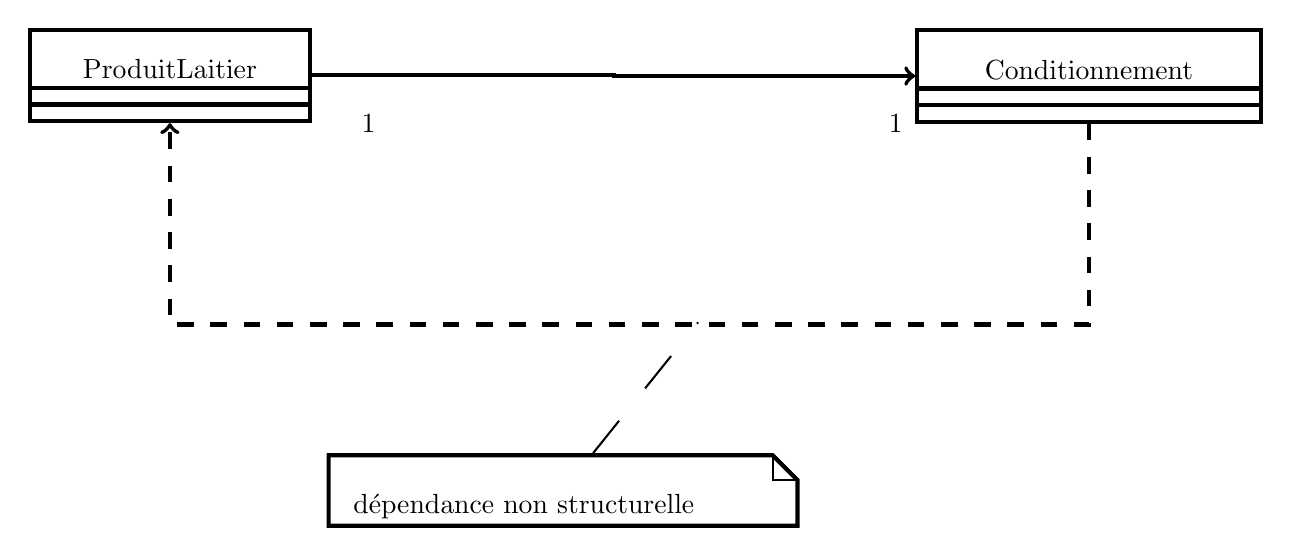
\begin{tikzpicture}
\pgftransformxscale{1.000000}
\pgftransformyscale{-1.000000}
\definecolor{dialinecolor}{rgb}{0.000000, 0.000000, 0.000000}
\pgfsetstrokecolor{dialinecolor}
\definecolor{dialinecolor}{rgb}{1.000000, 1.000000, 1.000000}
\pgfsetfillcolor{dialinecolor}
\pgfsetlinewidth{0.100000\du}
\pgfsetdash{}{0pt}
\definecolor{dialinecolor}{rgb}{1.000000, 1.000000, 1.000000}
\pgfsetfillcolor{dialinecolor}
\fill (9.500000\du,-10.487500\du)--(9.500000\du,-9.087500\du)--(16.252500\du,-9.087500\du)--(16.252500\du,-10.487500\du)--cycle;
\definecolor{dialinecolor}{rgb}{0.000000, 0.000000, 0.000000}
\pgfsetstrokecolor{dialinecolor}
\draw (9.500000\du,-10.487500\du)--(9.500000\du,-9.087500\du)--(16.252500\du,-9.087500\du)--(16.252500\du,-10.487500\du)--cycle;
% setfont left to latex
\definecolor{dialinecolor}{rgb}{0.000000, 0.000000, 0.000000}
\pgfsetstrokecolor{dialinecolor}
\node at (12.876250\du,-9.537500\du){ProduitLaitier};
\definecolor{dialinecolor}{rgb}{1.000000, 1.000000, 1.000000}
\pgfsetfillcolor{dialinecolor}
\fill (9.500000\du,-9.087500\du)--(9.500000\du,-8.687500\du)--(16.252500\du,-8.687500\du)--(16.252500\du,-9.087500\du)--cycle;
\definecolor{dialinecolor}{rgb}{0.000000, 0.000000, 0.000000}
\pgfsetstrokecolor{dialinecolor}
\draw (9.500000\du,-9.087500\du)--(9.500000\du,-8.687500\du)--(16.252500\du,-8.687500\du)--(16.252500\du,-9.087500\du)--cycle;
\definecolor{dialinecolor}{rgb}{1.000000, 1.000000, 1.000000}
\pgfsetfillcolor{dialinecolor}
\fill (9.500000\du,-8.687500\du)--(9.500000\du,-8.287500\du)--(16.252500\du,-8.287500\du)--(16.252500\du,-8.687500\du)--cycle;
\definecolor{dialinecolor}{rgb}{0.000000, 0.000000, 0.000000}
\pgfsetstrokecolor{dialinecolor}
\draw (9.500000\du,-8.687500\du)--(9.500000\du,-8.287500\du)--(16.252500\du,-8.287500\du)--(16.252500\du,-8.687500\du)--cycle;
\pgfsetlinewidth{0.100000\du}
\pgfsetdash{}{0pt}
\definecolor{dialinecolor}{rgb}{1.000000, 1.000000, 1.000000}
\pgfsetfillcolor{dialinecolor}
\fill (30.880000\du,-10.472500\du)--(30.880000\du,-9.072500\du)--(39.152500\du,-9.072500\du)--(39.152500\du,-10.472500\du)--cycle;
\definecolor{dialinecolor}{rgb}{0.000000, 0.000000, 0.000000}
\pgfsetstrokecolor{dialinecolor}
\draw (30.880000\du,-10.472500\du)--(30.880000\du,-9.072500\du)--(39.152500\du,-9.072500\du)--(39.152500\du,-10.472500\du)--cycle;
% setfont left to latex
\definecolor{dialinecolor}{rgb}{0.000000, 0.000000, 0.000000}
\pgfsetstrokecolor{dialinecolor}
\node at (35.016250\du,-9.522500\du){Conditionnement};
\definecolor{dialinecolor}{rgb}{1.000000, 1.000000, 1.000000}
\pgfsetfillcolor{dialinecolor}
\fill (30.880000\du,-9.072500\du)--(30.880000\du,-8.672500\du)--(39.152500\du,-8.672500\du)--(39.152500\du,-9.072500\du)--cycle;
\definecolor{dialinecolor}{rgb}{0.000000, 0.000000, 0.000000}
\pgfsetstrokecolor{dialinecolor}
\draw (30.880000\du,-9.072500\du)--(30.880000\du,-8.672500\du)--(39.152500\du,-8.672500\du)--(39.152500\du,-9.072500\du)--cycle;
\definecolor{dialinecolor}{rgb}{1.000000, 1.000000, 1.000000}
\pgfsetfillcolor{dialinecolor}
\fill (30.880000\du,-8.672500\du)--(30.880000\du,-8.272500\du)--(39.152500\du,-8.272500\du)--(39.152500\du,-8.672500\du)--cycle;
\definecolor{dialinecolor}{rgb}{0.000000, 0.000000, 0.000000}
\pgfsetstrokecolor{dialinecolor}
\draw (30.880000\du,-8.672500\du)--(30.880000\du,-8.272500\du)--(39.152500\du,-8.272500\du)--(39.152500\du,-8.672500\du)--cycle;
\pgfsetlinewidth{0.100000\du}
\pgfsetdash{}{0pt}
\definecolor{dialinecolor}{rgb}{1.000000, 1.000000, 1.000000}
\pgfsetfillcolor{dialinecolor}
\fill (16.700000\du,-0.237500\du)--(27.395000\du,-0.237500\du)--(27.995000\du,0.362500\du)--(27.995000\du,1.462500\du)--(16.700000\du,1.462500\du)--cycle;
\definecolor{dialinecolor}{rgb}{0.000000, 0.000000, 0.000000}
\pgfsetstrokecolor{dialinecolor}
\draw (16.700000\du,-0.237500\du)--(27.395000\du,-0.237500\du)--(27.995000\du,0.362500\du)--(27.995000\du,1.462500\du)--(16.700000\du,1.462500\du)--cycle;
\pgfsetlinewidth{0.050000\du}
\definecolor{dialinecolor}{rgb}{0.000000, 0.000000, 0.000000}
\pgfsetstrokecolor{dialinecolor}
\draw (27.395000\du,-0.237500\du)--(27.395000\du,0.362500\du)--(27.995000\du,0.362500\du);
% setfont left to latex
\definecolor{dialinecolor}{rgb}{0.000000, 0.000000, 0.000000}
\pgfsetstrokecolor{dialinecolor}
\node[anchor=west] at (17.050000\du,1.007500\du){dépendance non structurelle};
\pgfsetlinewidth{0.100000\du}
\pgfsetbuttcap
\pgfsetdash{}{0pt}
{
\definecolor{dialinecolor}{rgb}{0.000000, 0.000000, 0.000000}
\pgfsetfillcolor{dialinecolor}
% was here!!!
\pgfsetarrowsend{to}
\definecolor{dialinecolor}{rgb}{0.000000, 0.000000, 0.000000}
\pgfsetstrokecolor{dialinecolor}
\draw (16.302918\du,-9.387500\du)--(23.566331\du,-9.387500\du)--(23.566331\du,-9.372500\du)--(30.829744\du,-9.372500\du);
}
% setfont left to latex
\pgfsetlinewidth{0.100000\du}
\pgfsetdash{{1.000000\du}{1.000000\du}}{0\du}
\pgfsetdash{{0.400000\du}{0.400000\du}}{0\du}
\pgfsetmiterjoin
\pgfsetbuttcap
{
\definecolor{dialinecolor}{rgb}{0.000000, 0.000000, 0.000000}
\pgfsetfillcolor{dialinecolor}
% was here!!!
\pgfsetarrowsend{to}
\definecolor{dialinecolor}{rgb}{0.000000, 0.000000, 0.000000}
\pgfsetstrokecolor{dialinecolor}
\draw (35.016250\du,-8.222185\du)--(35.016250\du,-3.387500\du)--(12.876250\du,-3.387500\du)--(12.876250\du,-8.237231\du);
}
% setfont left to latex
\pgfsetlinewidth{0.050000\du}
\pgfsetdash{{0.400000\du}{0.400000\du}}{0\du}
\pgfsetdash{{1.000000\du}{1.000000\du}}{0\du}
\pgfsetbuttcap
{
\definecolor{dialinecolor}{rgb}{0.000000, 0.000000, 0.000000}
\pgfsetfillcolor{dialinecolor}
% was here!!!
\definecolor{dialinecolor}{rgb}{0.000000, 0.000000, 0.000000}
\pgfsetstrokecolor{dialinecolor}
\draw (23.070498\du,-0.287775\du)--(25.600000\du,-3.437500\du);
}
% setfont left to latex
\definecolor{dialinecolor}{rgb}{0.000000, 0.000000, 0.000000}
\pgfsetstrokecolor{dialinecolor}
\node[anchor=west] at (17.250000\du,-8.237500\du){1};
% setfont left to latex
\definecolor{dialinecolor}{rgb}{0.000000, 0.000000, 0.000000}
\pgfsetstrokecolor{dialinecolor}
\node[anchor=west] at (29.950000\du,-8.237500\du){1};
\end{tikzpicture}
